% fig_halow_tcp_throughput.tex — Caudal TCP simétrico por ancho de banda HaLow
% Datos: thesis_symmetric_package (Feb 2025, Laboratorio UNAL)
% v2 — Espaciado mejorado, barras más anchas, leyenda reubicada
\begin{figure}[htbp]
\centering
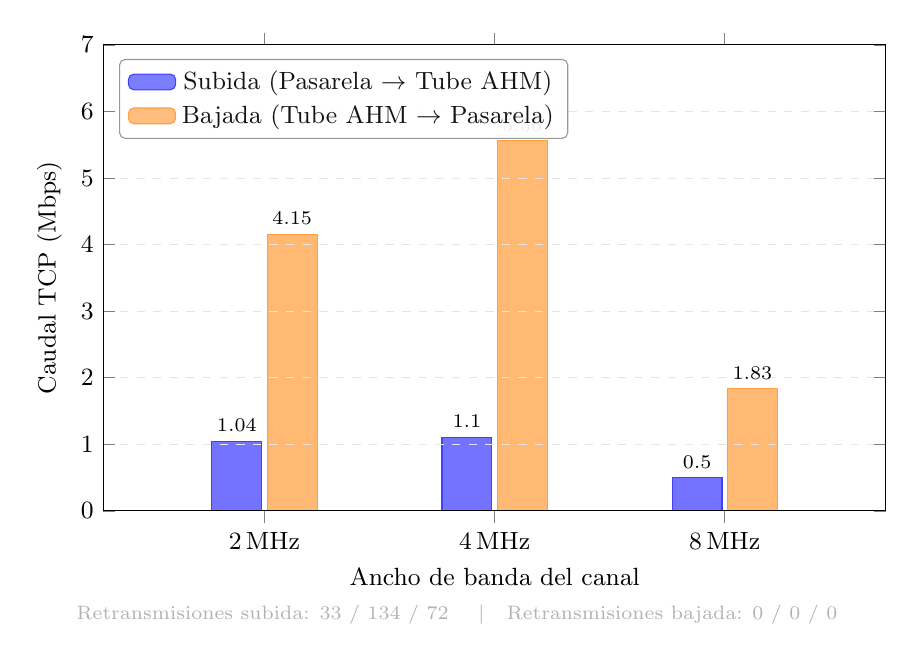
\begin{tikzpicture}
\begin{axis}[
    ybar,
    width=0.95\textwidth,
    height=7.5cm,
    bar width=18pt,
    enlarge x limits=0.35,
    ylabel={Caudal TCP (Mbps)},
    xlabel={Ancho de banda del canal},
    symbolic x coords={2\,MHz, 4\,MHz, 8\,MHz},
    xtick=data,
    ymin=0, ymax=7,
    ytick={0,1,2,3,4,5,6,7},
    legend style={at={(0.02,0.97)}, anchor=north west, legend columns=1, font=\small,
                  draw=black!40, fill=white, fill opacity=0.92, rounded corners=2pt},
    nodes near coords,
    every node near coord/.append style={font=\scriptsize\bfseries, /pgf/number format/fixed,
                                          /pgf/number format/precision=2},
    major grid style={gray!20, dashed},
    ymajorgrids=true,
    tick label style={font=\small},
    label style={font=\small},
    axis on top,
    area legend,
]

% Subida (Pasarela → Tube AHM)
\addplot[fill=blue!55, draw=blue!75] coordinates {
    (2\,MHz, 1.044)
    (4\,MHz, 1.100)
    (8\,MHz, 0.497)
};

% Bajada (Tube AHM → Pasarela)
\addplot[fill=orange!55, draw=orange!75] coordinates {
    (2\,MHz, 4.153)
    (4\,MHz, 5.558)
    (8\,MHz, 1.833)
};

\legend{Subida (Pasarela $\rightarrow$ Tube AHM), Bajada (Tube AHM $\rightarrow$ Pasarela)}

\end{axis}

% Anotación de retransmisiones
\node[anchor=north, font=\scriptsize, text=gray!60, align=center] at (current bounding box.south) {%
    Retransmisiones subida: 33 / 134 / 72 \quad$|$\quad Retransmisiones bajada: 0 / 0 / 0};

\end{tikzpicture}
\caption[Caudal TCP por ancho de banda HaLow]{Caudal TCP medido por ancho de banda del canal IEEE~802.11ah.
La bajada (Tube AHM $\rightarrow$ Pasarela) supera a la subida entre 3$\times$ y 5$\times$ debido a la mayor potencia de transmisi\'{o}n del AP.
Prueba \texttt{iperf3} con flujo TCP de 30\,s por direcci\'{o}n.
El canal de 4\,MHz ofrece el mejor rendimiento (5{,}56\,Mbps bajada)
mientras que 8\,MHz presenta degradaci\'{o}n severa.}
\label{fig:halow-tcp-throughput}
\end{figure}
